% chapter_13_HLT.tex -- chapter 13 of the JitJet book: the High Level Trigger, the second checkpoint (Rule G of the
% Constitution: B1, B2, one section per step, B4, B5). ONE sample: the event with its pileup (Rule H).
% Every number comes from test/13_HLT/out/ (ledger_13_HLT.txt, hlt_13_HLT.log, menu_13_HLT.txt, step5_HLT_13_HLT.log,
% the PNG pages); the companion doc/chapter/chapter_13_HLT.md lists them.

\chapter{13 -- HLT: the High Level Trigger reconstructs the event and keeps it}
\label{ch:13_HLT}

\section{What this chapter is about}

The Level-1 trigger of chapter~\ref{ch:12_L1T} said yes. In the detector that answer travels back to every readout
board, which sends its piece of the event to the data acquisition; an \emph{event builder} assembles the pieces, and
the complete event, about two megabytes of raw data, is handed to one computer of the \emph{High Level Trigger}
(HLT) farm. The HLT is the second and last checkpoint of the journey. Unlike the Level-1 trigger it is software: the
same CMSSW as the offline reconstruction, in faster versions, running on commercial computers with graphics cards. It
receives up to about $100\,000$ events per second from the Level-1 trigger and keeps a per cent or so of them: those
are the events that are written to disk and that an analysis will ever see.

The program of the HLT is the \emph{menu}, a list of \emph{paths}. A path is a sequence of modules: producers that
reconstruct something (hits, tracks, jets) and filters that cut on it. A path stops at the first filter that fails;
the event is kept if at least one path runs to its end. Every path starts with the question of chapter~\ref{ch:12_L1T},
``did my Level-1 seed fire?'', so that the farm reconstructs only what the Level-1 decision justifies, and modules
shared by many paths run once per event. The menu of this chapter, the 2025 menu of CMSSW\_15\_0\_5, has 898
paths. Its \emph{path of the book} is \code{HLT\_PFJet110}, the jet path that the seed \code{L1\_SingleJet90} of
chapter~\ref{ch:12_L1T} opens (figure~\ref{fig:13_path}). We follow it in five steps:

\begin{enumerate}
\item \textbf{the raw event, the Level-1 seed and the prescale}: the event as bytes; the Level-1 record unpacked; the
seed and prescale modules that open or close each path;
\item \textbf{calorimeter jets}: the ECAL and HCAL energies reconstructed, summed into towers, clustered into jets of
radius 0.4, corrected; a first, cheap cut on them;
\item \textbf{tracking and vertices}: the charged particles reconstructed from the pixel and strip hits, and the
collision points along the beam;
\item \textbf{particle flow and PF jets}: tracks and calorimeter clusters combined into a list of particles, and the
jets made of them, corrected;
\item \textbf{the decision of the paths}: the last filters, which of the 898 paths accept the event, and where it is
written: the datasets and the streams.
\end{enumerate}

\begin{figure}[!htb]
\centering
\begin{tikzpicture}[x=0.0905cm, y=1cm, font=\scriptsize]
% the 174 modules of HLT_PFJet110 in the order they run, as a bar (one unit = one module)
\foreach \a/\b/\c in {0/5/black!25, 5/7/orange!70, 7/22/green!30, 22/35/green!55, 35/53/blue!12, 53/63/blue!25,
  63/73/blue!12, 73/78/blue!40, 78/118/blue!12, 118/142/blue!40, 142/159/red!25, 159/171/red!45, 171/174/orange!70}
{ \fill[\c, draw=black!60, line width=0.3pt] (\a,0) rectangle (\b,2.0); }
\foreach \x/\t in {2.5/{L1 record}, 14.5/{calo hits}, 28.5/{calo jets}, 44/{muon hits}, 58/{Si hits}, 68/{L3 muons},
  75.5/{pixel tracks}}
{ \node[rotate=90, font=\tiny] at (\x,1.0) {\t}; }
\foreach \x/\t in {98/{L3 muons}, 130/{full tracks}, 150.5/{PF}, 165/{PF jets}}
{ \node at (\x,1.0) {\t}; }
\draw[->, >={Stealth[length=1.5mm]}] (6,-0.75) node[below, align=center] {seed, prescale\\(5, 6)} -- (6,-0.05);
\draw[->, >={Stealth[length=1.5mm]}] (32.5,-0.75) node[below, align=center] {calo cut $80\GeV$\\(32)} -- (32.5,-0.05);
\draw[->, >={Stealth[length=1.5mm]}] (172.5,-0.75) node[below left=0pt and -6pt, align=right] {PF cut $110\GeV$\\(172)} -- (172.5,-0.05);
\foreach \x in {0,25,50,75,100,125,150,174} \node[text=black!60] at (\x,2.25) {\x};
\node[anchor=west, text=black!60] at (0,2.65) {module number in \code{HLT\_PFJet110\_v13}};
\foreach \a/\b/\t in {0/7/{step 1}, 7/35/{step 2}, 35/142/{step 3 (and the muons)}, 142/174/{steps 4 and 5}}
{ \draw[black!50] (\a+0.3,-1.75) -- (\b-0.3,-1.75); \node[below] at ({(\a+\b)/2},-1.75) {\t}; }
\end{tikzpicture}
\caption{The path of the book, \code{HLT\_PFJet110}, module by module (\code{menu\_13\_HLT.txt}, section 2): 174
modules, of which the seed and the prescale are numbers 5 and 6, the cut on the calorimeter jets number 32 and the
cut on the PF jets number 172. Light blue: the reconstruction of the muons, which particle flow needs (68 modules).
Most of the path is shared with other paths and runs once per event.}
\label{fig:13_path}
\end{figure}

\begin{table}[!htb]
\centering\small\setlength{\tabcolsep}{4pt}
\caption{The five steps at a glance, for our event (\code{ledger\_13\_HLT.txt}).}
\label{tab:13_glance}
\begin{tabular}{@{}c>{\raggedright\arraybackslash}p{4.6cm}>{\raggedright\arraybackslash}p{4.2cm}>{\raggedright\arraybackslash}p{5.3cm}@{}}
\toprule
step & modules (examples) & what it makes & in our event \\
\midrule
1 & \code{hltGtStage2Digis}, \code{hltL1sSingleJet90}, \code{hltPrePFJet110} & the Level-1 record; for each path: go or stop & 1\,906\,128 bytes from 678 boards; 652 of 754 paths stop at their seed \\
2 & \code{hltTowerMakerForAll}, \code{hltAK4CaloJetsCorrected} & 2051 towers, calo jets & 2 jets above $30\GeV$: $118.5$ and $93.3\GeV$ \\
3 & \code{hltPixelTracks}, \code{hltMergedTracks}, \code{hltVerticesPF} & pixel tracks, full tracks, vertices & 2981 pixel tracks, 116 full tracks, 1 vertex: the signal \\
4 & \code{hltParticleFlow}, \code{hltAK4PFJetsCorrected} & 1366 particles, PF jets & 2 jets above $30\GeV$: $126.7$ and $86.7\GeV$ \\
5 & \code{hltSinglePFJet110}, \code{TriggerResults} & the decision of every path & 40 paths accept; \code{HLT\_PFJet110} by $16.7\GeV$ \\
\bottomrule
\end{tabular}
\end{table}

One event is followed (\path{test/13_HLT/run_13_HLT.sh}), the same as in chapter~\ref{ch:12_L1T}: the signal with
the 71, 68 and 54 collisions of bunch crossings $-1$, 0 and $+1$ (Rule H). Who made an object is read from the truth
the file still carries: the two generator jets of chapter~\ref{ch:07_GenJet}, the simulated position of every
collision along the beam (\code{addPileupInfo}, \code{genParticles:xyz0}).

\section{From the previous chapter}

One file of chapter~\ref{ch:12_L1T} enters (Rule E), \path{test/12_L1T/out/step4_L1_12_L1T.root}: the digis of
chapter~\ref{ch:11_DIGI} and the products of the Level-1 emulator, $12.3\,$MB. The decision it carries: 63 of the 465
Level-1 algorithms fired, among them \code{L1\_SingleJet90}, by $46\GeV$ on the $\bar b$ jet in the HF ($136.0\GeV$)
and by $18.5\GeV$ on the $b$ jet ($108.5\GeV$). That algorithm is the seed of \code{HLT\_PFJet110}: the door
through which the event enters this chapter.

The HLT does not read digis. It reads what the detector sends: \emph{raw data}, one block of bytes per readout board
(a FED, ``front-end driver''). The first part of the job of this chapter (\code{cmsDriver.py -s DIGI2RAW,HLT:@relval2025})
therefore packs the digis and the Level-1 record into raw data, as the readout would (\code{DIGI2RAW},
table~\ref{tab:13_packers}); the HLT then unpacks them again. Packing is not a copy: each packer writes the format of
its board, with headers, trailers and the zero suppression of the hardware, and the size of each block is what the
readout links have to carry. In production the Level-1 emulation and \code{DIGI2RAW} run in the same job, and three products
of the Level-1 job that the packers read were not kept by chapter~\ref{ch:12_L1T}; they are remade, with the same
configuration, at the head of the job (the companion, section~1). Nothing is added to the event: the digis are those
of chapter~\ref{ch:11_DIGI}, the Level-1 decision is that of chapter~\ref{ch:12_L1T}.

\begin{table}[!htb]
\centering\small
\caption{From the previous chapter: the packers of \code{DIGI2RAW}, the reverse of the unpackers that open every HLT
path (\code{step5\_HLT\_13\_HLT\_cfg.py}, the path \code{digi2raw\_step}, whose first three modules, not listed, are the
Level-1 products remade at the head of the job).}
\label{tab:13_packers}
\begin{tabular}{@{}>{\raggedright\arraybackslash}p{5.3cm}>{\raggedright\arraybackslash}p{4.2cm}>{\raggedright\arraybackslash}p{5.9cm}@{}}
\toprule
module & C++ type & packs \\
\midrule
\code{siPixelRawData}, \code{SiStripDigiToRaw} & \code{SiPixelDigiToRaw}, \ldots & the pixel and strip digis of chapter~\ref{ch:11_DIGI} \\
\code{ecalPacker}, \code{esDigiToRaw} & \code{EcalDigiToRaw}, \code{ESDigiToRaw} & ECAL data frames, selective-readout flags, ECAL trigger primitives; preshower \\
\code{hcalRawDatauHTR} & \code{HcalDigiToRawuHTR} & HB, HE, HF data frames and the HCAL trigger primitives \\
\code{cscpacker}, \code{dtpacker}, \code{rpcpacker}, \code{gemPacker} & & the muon digis and the CSC trigger primitives \\
\code{caloLayer1RawFed1354}, \code{1356}, \code{1358} & \code{L1TDigiToRaw} & the inputs and towers of calorimeter Layer-1 \\
\code{caloStage2Raw}, \code{bmtfStage2Raw}, \code{omtfStage2Raw}, \code{gmtStage2Raw} & & Layer-2 objects, track-finder candidates, $\mu$GMT muons \\
\code{gtStage2Raw} & \code{L1TDigiToRaw} & the record of the global trigger: the 512 bits and the objects (FED 1404) \\
\code{rawDataCollector} & \code{RawDataCollectorByLabel} & all of it, one \code{FEDRawDataCollection} \\
\bottomrule
\end{tabular}
\end{table}

Which menu? The one the release gives the 2025 simulation: \code{HLT:@relval2025} is \code{2025v10}
(\path{Configuration/HLT/python/autoHLT.py}), the frozen menu \code{/frozen/2025/2e34/v1.0/HLT/V2} of the 2025 data
taking (\path{HLTrigger/Configuration/python/HLT_2025v10_cff.py}), module for module the physics menu \code{GRun} of
the release. Its seeds name algorithms of the 2025 Level-1 menu of chapter~\ref{ch:12_L1T}, and every one exists:
\path{python/hltL1Menu_cff.py}, which checks the seeds against that menu, changes nothing, and the 898 paths run. (The
2024 version of this chapter ran the same menu on the 2024 Level-1 menu: 30 of the algorithms its seeds name did not
exist, and 37 paths had to be removed. The release has no 2024 HLT menu: \code{HLT:@relval2024} is a ``fake'' menu
of three paths.) The output adds to the input what the HLT made: $20.8\,$MB in all.

\section{Step 1: the raw event, the Level-1 seed and the prescale}

\textbf{What the step does.} The event arrives as 678 blocks of bytes, one per readout board that has data
(table~\ref{tab:13_raw}). More than half of it is the strip tracker, which has almost ten million channels; the calorimeters
are a fifth. Every path then starts with the same five modules (\code{HLTBeginSequence}): \code{hltTriggerType}
(is this a physics event?), \code{hltGtStage2Digis}, which unpacks the record of the Level-1 global trigger from its
board (FED 1404), \code{hltGtStage2ObjectMap}, which runs the global-trigger algorithm of chapter~\ref{ch:12_L1T}
once more on the unpacked objects to know \emph{which} objects satisfied each algorithm,
\code{hltOnlineMetaDataDigis} and \code{hltOnlineBeamSpot}, the position of the beam. Then come the two modules that decide whether the path runs at all.

\emph{The seed} (\code{HLTL1TSeed}, 224 of them in the menu) holds a logical expression of Level-1 algorithm names,
\code{L1SeedsLogicalExpression}; for \code{HLT\_PFJet110} it is \code{"L1\_SingleJet90"}. It reads the final
decision bit of each algorithm and evaluates the expression; if it is false the path stops there. If it is true the
seed also records the Level-1 objects that made the algorithm fire, so that a later module can look only where
the Level-1 trigger saw something (the electron and muon paths reconstruct in such \emph{regions}; the jet paths
reconstruct everywhere).

\emph{The prescaler} (\code{HLTPrescaler}, one per path, 893 in the menu) keeps one event in $N$ of those that reach
it. A path whose rate would be too high is not removed but prescaled: \code{HLT\_PFJet40} would fire on a large
fraction of all collisions, so in data taking it keeps only a small, known fraction of them, enough to measure the
jet trigger efficiency, while a path with a threshold high enough to fit in the bandwidth runs with $N=1$. The
values of $N$ are a table with one column per luminosity, loaded online by the \code{PrescaleService}.

\begin{plainwords}[The simulation runs without prescales, again]
The menu of the release is a \code{\_cff} file: the paths without the services of the online configuration. It has
no \code{PrescaleService} (\path{menu_13_HLT.txt}: ``no PrescaleService: every HLTPrescaler has prescale 1''), so,
as in chapter~\ref{ch:12_L1T}, every path runs unprescaled. In our event 0 of the 754 \code{HLT\_} and \code{DST\_}
paths is stopped by a prescaler. The question to ask of a simulated event is ``which paths accept it'', and then, for
the analysis one has in mind, whether those paths ran unprescaled in the data.
\end{plainwords}

\begin{plainwords}[How long it takes]
In this job, on one core of a processor without a graphics card, the HLT took about a minute to start (reading the
configuration of 4783 modules and the conditions of the global tag) and about six seconds for our event
(\path{step5_HLT_13_HLT.log}: from ``Begin processing'' at 13:23:46 to the closing of the input at 13:23:52), the first
event of the job, which also pays the initialisation of many modules. On the farm a process runs for days, the start
is paid once, the modules marked \code{@alpaka} run on the graphics cards, and the menu is designed so that the
average event takes a small fraction of a second. Our event is not average: it passes a jet seed, so the full
tracking and particle flow run.
\end{plainwords}

\textbf{The numbers of the event.} The record unpacked by the HLT is that of chapter~\ref{ch:12_L1T}, bit for bit:
63 algorithms fired, 9 jets, 12 e/$\gamma$, 12 $\tau$, one muon (figure~\ref{fig:13_seed}). Of the 754 physics
(\code{HLT\_}) and scouting (\code{DST\_}) paths, 652 stop at their seed: they cost the farm nothing but the
evaluation of an expression. 102 start their reconstruction. \code{hltL1sSingleJet90} is true and hands two Level-1
jets to the rest of its path, $136.0\GeV$ at $(\eta,\phi)=(-3.74,1.00)$ and $108.5\GeV$ at $(-1.52,-1.98)$: the two
jets of the signal. The seed of \code{HLT\_PFJet200}, \code{L1\_SingleJet120}, hands only the first; the seeds of the
paths above $200\GeV$ (\code{L1\_SingleJet180} and the like) are false.

\begin{table}[!htb]
\centering\small
\caption{Step 1: the raw event as the HLT receives it, by subsystem (\code{ledger\_13\_HLT.txt}, section 1; FED
numbers of \code{DataFormats/FEDRawData/interface/FEDNumbering.h}).}
\label{tab:13_raw}
\begin{tabular}{l rrr}
\toprule
subsystem & readout boards (FEDs) & kB & share \\
\midrule
strip tracker & 381 & 997.5 & 53.6\,\% \\
pixel tracker & 108 & 306.7 & 16.5\,\% \\
HCAL (HB, HE, HF, HO) & 44 & 240.6 & 12.9\,\% \\
ECAL preshower & 40 & 137.4 & 7.4\,\% \\
ECAL & 54 & 103.9 & 5.6\,\% \\
CSC & 36 & 46.9 & 2.5\,\% \\
Level-1 trigger & 7 & 27.1 & 1.5\,\% \\
GEM, DT, RPC & 8 & 1.3 & 0.1\,\% \\
\midrule
all & 678 & 1861.5 & \\
\bottomrule
\end{tabular}
\end{table}

\begin{figure}[!htb]
\centering
\includegraphics[width=0.93\textwidth]{13_HLT/out/hlt_13_HLT_seed_seed_run1_event1.png}
\caption{Step 1, what the HLT knows when a path starts: the Level-1 objects it unpacks
(\code{hlt\_13\_HLT\_seed\_seed\_run1\_event1.png}; squares: jets with their $E_{\mathrm T}$ in GeV, triangles: $\tau$,
dots: e/$\gamma$, star: the muon). The orange circles are the two jets that \code{hltL1sSingleJet90} records as the
reason it fired; magenta, the generator jets. The right panel: the raw data and the fate of the 754 paths.}
\label{fig:13_seed}
\end{figure}

\textbf{A path in the python of the menu.} The menu is a python file of $87\,551$ lines; our path is one of them,
and its first and last filters are two module definitions (\path{HLT_2025v10_cff.py}, shortened):

\begin{lstlisting}[style=py]
fragment.HLT_PFJet110_v13 = cms.Path( fragment.HLTBeginSequence + fragment.hltL1sSingleJet90
    + fragment.hltPrePFJet110 + fragment.HLTAK4CaloJetsSequence + fragment.hltSingleAK4CaloJet80
    + fragment.HLTAK4PFJetsSequence + fragment.hltPFJetsCorrectedMatchedToCaloJets80
    + fragment.hltSinglePFJet110 + fragment.HLTEndSequence )
fragment.hltL1sSingleJet90 = cms.EDFilter( "HLTL1TSeed",
    L1SeedsLogicalExpression = cms.string( "L1_SingleJet90" ), saveTags = cms.bool( True ), ... )
fragment.hltSinglePFJet110 = cms.EDFilter( "HLT1PFJet",
    inputTag = cms.InputTag( "hltPFJetsCorrectedMatchedToCaloJets80" ),
    MinPt = cms.double( 110.0 ), MaxEta = cms.double( 5.0 ), MinN = cms.int32( 1 ), ... )
\end{lstlisting}

\noindent The sequences (\code{HLTAK4CaloJetsSequence}, \code{HLTAK4PFJetsSequence}) expand into the modules of
figure~\ref{fig:13_path}: 209 entries, of which 174 distinct modules, since a sequence used twice brings modules that
have already run. The version suffix \code{\_v13} changes whenever the path changes; an analysis asks for
\code{HLT\_PFJet110\_v*}.

\textbf{What the seeds open.} The 102 paths that start are the ones the Level-1 decision of chapter~\ref{ch:12_L1T}
justifies, and they show what the HLT is for (table~\ref{tab:13_started}). Chapter~\ref{ch:12_L1T} found that 33 of
the 63 Level-1 algorithms needed an object the hard collision did not make: missing-energy seeds fired by an ETMHF
twice the neutrino, muon seeds fired by a pileup kaon, low-threshold jet and e/$\gamma$ seeds fired by the pileup of
the barrel. Those seeds open 30 missing-energy paths and 13 muon paths here. The HLT stops 29 of the 30
missing-energy paths, most of them at the first cut on the missing $H_{\mathrm T}$ of the calo jets
(\code{HLTMhtFilter}), and 12 of the 13 muon paths, which want a muon above 8, 10, 12 or $23\GeV$ (or two above
$50\GeV$). (With the 2024
settings the ring-28 jets of chapter~\ref{ch:12_L1T} had also opened 13 VBF and 6 multijet paths, all stopped here.) Reconstructing the event better than the Level-1 trigger could
is how the HLT brings the rate down by a factor of a hundred.

\begin{table}[!htb]
\centering\small
\caption{Step 1 and step 5: the 102 \code{HLT\_} and \code{DST\_} paths whose seed fired, by kind, and the filter types
that stopped them (\code{ledger\_13\_HLT.txt}, section 5).}
\label{tab:13_started}
\begin{tabular}{@{}l rr >{\raggedright\arraybackslash}p{7.2cm}@{}}
\toprule
kind of path & accepted & stopped & stopped by (C++ type of the filter) \\
\midrule
single jets, dijets & 16 & 14 & \code{HLT1PFJet} 4, \code{HLT1CaloJet} 4, \code{HLTDiPFJetAveEtaFilter} 4, \code{HLTDiCaloJetAveFilter} 2 \\
multijets, VBF, electrons & 0 & 0 & seeds not fired (2024: 6, 13 and 2 paths started, all stopped) \\
missing energy, $H_{\mathrm T}$ & 1 & 29 & \code{HLTMhtFilter} 16, \code{HLT1PFMET} 5, \code{HLTDeDxFilter} 3, \code{HLTHtMhtFilter} 2, others 3 \\
muons & 1 & 12 & \code{HLTMuonL2FromL1TPreFilter} 9, \code{HLTMuonL3PreFilter} 3 \\
scouting & 7 & 0 & \\
no object, L1 seed only, calibration & 15 & 0 & \\
isolated tracks, PPS, monitoring & 0 & 7 & \code{TriggerResultsFilter} 3, \code{HLTPixelIsolTrackL1TFilter} 2, \code{HLTPPSCalFilter} 2 \\
\midrule
all & 40 & 62 & \\
\bottomrule
\end{tabular}
\end{table}

\FloatBarrier
\section{Step 2: calorimeter jets}

\textbf{What the step does.} The paths that need jets first reconstruct the calorimeters, in four stages
(figure~\ref{fig:13_path}, modules 7 to 32).

\emph{Rec-hits.} The ECAL and HCAL boards are unpacked into digis, and a rec-hit is made of each digi: one energy and
one time per crystal or HCAL cell. The ECAL fits the ten samples of a crystal with a sum of pulse templates (the
``multifit''); the HCAL barrel and endcap do the same with eight samples (``MAHI''); the HF, whose signal is shorter
than 25\,ns, takes the charge of the one sample of the bunch crossing. These modules are written for graphics cards (their C++ type ends in
\code{@alpaka}); on a computer without one, as here, the same code runs on the processor.

\emph{Towers.} \code{hltTowerMakerForAll} (\code{CaloTowersCreator}) sums the rec-hits of each $\eta$--$\phi$ cell
into a tower, the same grid as the trigger towers of chapter~\ref{ch:12_L1T} (the towers 28 and 29 of the endcap are
separate here, and from $|i\eta|=21$ on a tower is $10^\circ$ wide). Only rec-hits above a threshold enter
(table~\ref{tab:13_towercuts}); the HO, the tail catcher outside the solenoid, is given the weight $10^{-99}$, that is
none.

\emph{Jets.} \code{hltAK4CaloJets} clusters the towers with the anti-$k_{\mathrm T}$ algorithm of radius 0.4, the
algorithm of the generator jets of chapter~\ref{ch:07_GenJet}, on every tower above $0.3\GeV$.
\code{hltAK4CaloJetsIDPassed} drops jets that look like noise (fewer than 2 rec-hits carrying 90\,\% of the energy).

\emph{Corrections.} A calorimeter jet measures less than the particles that made it, and pileup adds to it. The
jet energy corrections of the HLT, the payload \code{AK4CaloHLT} of the global tag
(\code{JetCorrectorParametersCollection\_Run3Winter24Digi\_AK4CaloHLT}), are applied in levels. \emph{L1FastJet}
subtracts the pileup: the energy density $\rho$, the median of $E_{\mathrm T}/\text{area}$ over a grid of
$0.55\times0.55$ cells of the whole event (\code{hltFixedGridRhoFastjetAllCalo}), times the area of the jet, with a
parametrised dependence on $\eta$ and \pt. \emph{L2Relative} makes the response flat in $\eta$ and \pt{} (the factor
that a simulated jet needs, on average, to come back to its generator jet). \emph{L3Absolute} and
\emph{L2L3Residual} are 1 in simulation (formula ``1'' in the payload). Each level is a formula of \pt, $\rho$ and the
area, with parameters in bins of $\eta$ (82 bins).

\begin{table}[!htb]
\centering\small
\caption{Step 2: the thresholds of the towers (\code{hltTowerMakerForAll}, \code{menu\_13\_HLT.txt}, section 3), in GeV.}
\label{tab:13_towercuts}
\begin{tabular}{@{}l>{\raggedright\arraybackslash}p{9.6cm}@{}}
\toprule
ECAL barrel & a crystal above 0.07; the ECAL sum of a tower above 0.2 \\
ECAL endcap & a crystal above 0.3; the ECAL sum of a tower above 0.45 \\
HCAL barrel & a cell above its threshold in the payload \code{HcalPFCuts\_2025\_mc} (\code{usePFThresholdsFromDB = True}); the python values 0.4 (depth 1), 0.3 are not used \\
HCAL endcap & the same payload; the python values 0.1 (depth 1), 0.2 are not used \\
HF & a long fibre above 0.5, a short fibre above 0.85 \\
HO & weight $10^{-99}$: not used \\
\bottomrule
\end{tabular}
\end{table}

\textbf{The numbers of the event.} The calorimeters give $11\,193$ rec-hits with $3198.9\GeV$ of transverse energy,
half of it in the HF ($1606.2\GeV$; table~\ref{tab:13_rechits}). The HF has the fewest cells and the most energy: its
1728 rec-hits hold $50.8\TeV$ of energy, the forward pileup at small angle, which is little transverse energy each.
The barrel ECAL has 956 rec-hits, half as many as with the 2024 settings: the higher zero suppression of
chapter~\ref{ch:11_DIGI}. The rec-hits make 2051 towers with $2842.9\GeV$ (barrel 342.8, endcap 882.9, HF
$1617.2\GeV$), close to the $2793\GeV$ of trigger primitives of chapter~\ref{ch:12_L1T}. The energy density is
$\rho=36.3\GeV$ per unit area: a jet of radius 0.4, area 0.50, collects $18\GeV$ of pileup on average. And so the
clustering finds 190 jets, 23 of them above $30\GeV$ before the corrections (figure~\ref{fig:13_calo}). After them,
two are left above $30\GeV$, and they are the two jets of the signal (table~\ref{tab:13_calojets}).

\begin{table}[!htb]
\centering\small
\caption{Step 2: the calorimeter rec-hits and towers of the event (\code{hlt\_13\_HLT.log}, lines \code{rechits} and
\code{towers}; $E_{\mathrm T}$ from the cell positions of the geometry).}
\label{tab:13_rechits}
\begin{tabular}{l rrrr c l rr}
\toprule
rec-hits & $n$ & $\sum E$ & $\sum E_{\mathrm T}$ & max $E_{\mathrm T}$ & & towers & $n$ & $\sum E_{\mathrm T}$ \\
\cmidrule(lr){1-5}\cmidrule(lr){7-9}
ECAL barrel & 956 & 208.3 & 142.6 & 3.01 & & barrel & 492 & 342.8 \\
ECAL endcap & 2515 & 2135.3 & 378.7 & 5.07 & & endcap & 771 & 882.9 \\
HCAL barrel & 2162 & 671.3 & 493.4 & 7.81 & & HF & 788 & 1617.2 \\
HCAL endcap & 3832 & 3028.3 & 578.0 & 9.63 & & all & 2051 & 2842.9 \\
HF & 1728 & 50\,809.4 & 1606.2 & 61.15 & & \quad EM / HAD & & 1090.3 / 1752.6 \\
\bottomrule
\end{tabular}
\end{table}

\begin{table}[!htb]
\centering\small
\caption{Step 2: the two signal jets as AK4 calo jets, level by level (\code{hlt\_13\_HLT.log}, lines \code{CaloJet};
the factors are recomputed from the payload and agree with \code{hltAK4CaloJetsCorrected}). A jet of the pileup for
comparison.}
\label{tab:13_calojets}
\begin{tabular}{@{}l rrr@{}}
\toprule
 & $b$ jet & $\bar b$ jet (HF) & a pileup jet \\
\midrule
generator jet \pt{} (visible) & 117.8 (79.8) & 115.9 & -- \\
calo jet $\eta$, $\phi$ & $-1.58$, $-2.08$ & $-3.72$, $0.96$ & $3.66$, $-0.36$ \\
towers, EM fraction & 33, 0.56 & 17, 0.27 & 16, 0.35 \\
raw \pt{} & 70.9 & 163.5 & 39.5 \\
after L1FastJet & 57.4 ($\times0.809$) & 119.9 ($\times0.734$) & 10.3 ($\times0.260$) \\
after L2Relative & \textbf{93.3} ($\times1.627$) & \textbf{118.5} ($\times0.987$) & \textbf{12.5} ($\times1.218$) \\
Level-1 jet of chapter~\ref{ch:12_L1T} & 108.5 & 136.0 & -- \\
\bottomrule
\end{tabular}
\end{table}

\emph{The $b$ jet} has $70.9\GeV$ of towers for $79.8\GeV$ of visible particles, pileup included: the calorimeter
response to hadrons is well below one. The pileup subtraction takes $13.5\GeV$ and the relative correction multiplies
by 1.63, to $93.3\GeV$. \emph{The $\bar b$ jet} in the HF has the opposite problem: $163.5\GeV$ of towers for a jet of
$115.9\GeV$, pileup and the HF response together; the subtraction takes $43.6\GeV$ (the area, the $\rho$ and the
parameters of this $\eta$ bin), and the relative correction is close to one. The pileup jets lose three quarters of
their energy to L1FastJet: what they are made of is exactly the $\rho$ that is subtracted.

The cut of the step is a single line of the menu: \code{hltSingleAK4CaloJet80}, at least one corrected calo jet
with $\pt\geq80\GeV$ and $\abseta<5$. Both signal jets pass. It costs a few milliseconds and protects what follows:
a path whose calo jets are too soft stops here, before the tracking.

\begin{figure}[!htb]
\centering
\includegraphics[width=0.93\textwidth]{13_HLT/out/hlt_13_HLT_calo_towers_run1_event1.png}
\caption{Step 2, the calorimeter towers of the event with the corrected AK4 calo jets above $20\GeV$ (red dashed
circles, \pt{} in GeV) and the generator jets (magenta) (\code{hlt\_13\_HLT\_calo\_towers\_run1\_event1.png}). The
grid is that of the trigger towers of chapter~\ref{ch:12_L1T}; a tower of $10^\circ$ or $20^\circ$ is shared over the
$5^\circ$ cells it covers. The bright bands at $\abseta\approx2.7$--3 and the HF are the pileup.}
\label{fig:13_calo}
\end{figure}

\begin{figure}[!htb]
\centering
\includegraphics[width=0.49\textwidth,trim=0 0 475 0,clip]{13_HLT/out/hlt_13_HLT_calo_jet1_run1_event1.png}\hfill
\includegraphics[width=0.49\textwidth,trim=0 0 475 0,clip]{13_HLT/out/hlt_13_HLT_calo_jet2_run1_event1.png}
\caption{Step 2, the towers around the two signal jets, $E_{\mathrm T}$ in GeV (\code{hlt\_13\_HLT\_calo\_jet1/jet2\_run1\_event1.png}).
Left: the $b$ jet; right: the $\bar b$ jet in the HF. The red dashed square is the $9\times9$ window of the
Level-1 jet of chapter~\ref{ch:12_L1T} nearest to the calo jet (for the $b$ jet centred on its seed,
$(i\eta,i\phi)=(-18,50)$, one tower away in both from the calo jet at $(-19,49)$; for the $\bar b$ jet both at
$(-34,12)$): in the same window the HLT towers hold $77.7\GeV$ for the $b$ jet (Layer-1: $74.5\GeV$) and
$215.9\GeV$ for the $\bar b$ jet (Layer-1: $189.0\GeV$).}
\label{fig:13_calozoom}
\end{figure}

\FloatBarrier
\section{Step 3: tracking and vertices}

\textbf{What the step does.} Tracking is the most expensive part of the HLT, and the menu does it in a careful order
(figure~\ref{fig:13_path}, modules 53 to 141).

\emph{Pixel tracks.} The pixel hits are clustered and given a position (\code{hltSiPixelClusters},
\code{hltSiPixelRecHits}); a \emph{cellular automaton} (\code{hltPixelTracksSoA}) links hits of three or four pixel
layers into short tracks, above $0.9\GeV$, with a helix fit. Pixel tracks are fast, but four points give a modest
momentum resolution.

\emph{Pixel vertices.} The pixel tracks above $0.5\GeV$ are clustered in $z$ into vertices (\code{hltPixelVertices}),
which are ordered by the sum of $\pt^2$ of their tracks: the first one is the \emph{primary vertex}, assumed to be
the interesting collision. \code{hltTrimmedPixelVertices} then keeps only the vertices whose sum of $\pt^2$ is at least
30\,\% of the first one (\code{fractionSumPt2 = 0.3}).

\emph{Full tracks.} Iteration 0 (\code{hltIter0PFLowPixelSeedsFromPixelTracks}) takes as seeds the pixel tracks that
point to a trimmed vertex (within $0.3\cm$ in $z$ and $0.1\cm$ in $r$), extends them through the ten layers of the
strip tracker with \code{mkFit} (a vectorised pattern recognition), fits them again and keeps the high-purity ones. A
second iteration, the \emph{doublet recovery}, seeds with pairs of pixel hits that iteration 0 did not use, for the
tracks that crossed only two pixel layers. The two are merged (\code{hltMergedTracks}), and the vertices of particle
flow are fitted from them (\code{hltVerticesPF}, deterministic annealing in $z$ and an adaptive fit).

\begin{plainwords}[Why the HLT reconstructs one collision of 69]
A bunch crossing of our event holds 69 collisions. Full tracking of all of them would take most of the time budget
of the farm. The HLT therefore reconstructs everything cheaply with pixels, decides which collision is the
interesting one (the vertex with the largest $\sum\pt^2$, because a hard scattering makes harder tracks than a
pileup collision) and builds full tracks only from the pixel tracks that come from it, and from vertices almost as
hard. In our event the trimming keeps one vertex out of 31, and it is the signal. The pileup collisions remain pixel
tracks, except those within the $3\mm$ seeding window around it. This works when the hard collision has hard charged particles in the tracker; an event whose jets are both
outside the tracker would have its primary vertex chosen among the pileup.
\end{plainwords}

\textbf{The numbers of the event.} The tracker gives $20\,925$ pixel clusters and $115\,249$ strip clusters. The
cellular automaton makes 2981 pixel tracks, of which 156 above $10\GeV$; they form 31 pixel vertices, for the 68
in-time pileup collisions and the signal. The first pixel vertex is at $z=3.107\cm$, with 40 pixel tracks: the signal,
whose simulated vertex is at $z=3.112\cm$ (no pileup collision is within a millimetre of it). It is the only vertex
the trimming keeps. Iteration 0 builds 108 tracks, the doublet recovery 8 more: 116 full tracks, 49 of them above
$1\GeV$, with on average 4.0 pixel and 9.3 strip hits. They make one PF vertex, at $z=3.111\cm$, $7\um$ from the
simulated one (the pixel vertex was $53\um$ away), with 107 tracks; 61 tracks with $121.8\GeV$ are within a millimetre of it
(figure~\ref{fig:13_track}). Another 27 are within a millimetre of pixel vertex 8, a pileup collision $2.2\mm$ away,
inside the $3\mm$ window of iteration 0.

\begin{table}[!htb]
\centering\small
\caption{Step 3: the tracking of the HLT, stage by stage, for our event (\code{hlt\_13\_HLT.log}, lines \code{clusters},
\code{tracks}, \code{vertices}; the cuts from \code{menu\_13\_HLT.txt}, section 3).}
\label{tab:13_tracking}
\begin{tabular}{@{}>{\raggedright\arraybackslash}p{4.9cm}>{\raggedright\arraybackslash}p{6.6cm} r@{}}
\toprule
stage (module) & what it does, with which cuts & our event \\
\midrule
pixel and strip clusters & neighbouring channels above threshold & 20\,925 / 115\,249 \\
pixel tracks (\code{hltPixelTracks}) & cellular automaton, 3 or 4 pixel hits, $\pt>0.9\GeV$ & 2981 \\
pixel vertices (\code{hltPixelVertices}) & clusters in $z$ of pixel tracks above $0.5\GeV$ & 31 \\
kept vertices (\code{hltTrimmedPixelVertices}) & $\sum\pt^2\geq0.3\times$ the first vertex & 1 \\
iteration 0 & seeds: pixel tracks within $0.3\cm$ in $z$ of a kept vertex; \code{mkFit}; high purity & 108 \\
doublet recovery & seeds: pixel pairs in regions of inactive pixel modules & 8 \\
merged (\code{hltMergedTracks}) & the two, without duplicates & 116 \\
PF vertices (\code{hltVerticesPF}) & deterministic annealing in $z$, adaptive fit & 1 \\
\bottomrule
\end{tabular}
\end{table}

\emph{The pileup vertices.} Each pixel vertex can be compared with the simulated collisions (table~\ref{tab:13_vertices}):
the first ten are each within $80\um$ of a simulated collision, most within $40\um$. The HLT knows where the pileup
collisions are; it only does not build their full tracks. Only the first vertex is kept: no other pixel vertex reaches 30\,\% of its
$\sum\pt^2$.

\begin{table}[!htb]
\centering\small
\caption{Step 3: the first ten pixel vertices, in the order of the HLT, and the simulated collision nearest to each in
$z$ (\code{hlt\_13\_HLT.log}, lines \code{vertex pixel}; ``pu$k$'' is the $k$-th in-time pileup collision of
\code{addPileupInfo}).}
\label{tab:13_vertices}
\begin{tabular}{r rrl r}
\toprule
& $z$ [cm] & pixel tracks & nearest simulated collision & $\Delta z$ [$\mu$m] \\
\midrule
0 & 3.1066 & 40 & the signal & 53 \\
1 & $-0.3305$ & 22 & pu9 & 79 \\
2 & $-5.4560$ & 31 & pu30 & 17 \\
3 & 2.0815 & 22 & pu42 & 12 \\
4 & 0.3620 & 27 & pu35 & 16 \\
5 & $-2.0472$ & 13 & pu51 & 3 \\
6 & $-2.8665$ & 18 & pu29 & 9 \\
7 & 2.4981 & 25 & pu22 & 34 \\
8 & 2.8856 & 20 & pu34 & 64 \\
9 & 1.4886 & 28 & pu10 & 39 \\
\bottomrule
\end{tabular}
\end{table}

\emph{The two jets.} Inside the $b$ jet ($\Delta R<0.4$) there are 7 tracks with $50.1\GeV$, six of them from the
signal vertex; the charged particles of the generator jet have $32.6\GeV$. Two tracks more than with the 2024
settings: the electron of the $B^-$ decay ($5.0\GeV$) and a track of $11.2\GeV$ a hair ($\Delta R=0.04$) from the
pion of $11.0\GeV$, with no simulated particle of its own: a duplicate, or a secondary; which is not established. The $\bar b$ jet, at $\eta=-3.75$, is
outside the tracker ($\abseta<2.5$): its $44.0\GeV$ of charged particles leave no track. For the HLT this jet will be
calorimeter only, in step~4 as in step~2.

\begin{figure}[!htb]
\centering
\includegraphics[width=0.49\textwidth,trim=0 0 475 0,clip]{13_HLT/out/hlt_13_HLT_track_etaphi_run1_event1.png}\hfill
\includegraphics[width=0.49\textwidth,trim=0 0 475 0,clip]{13_HLT/out/hlt_13_HLT_track_vertices_run1_event1.png}
\caption{Step 3 (\code{hlt\_13\_HLT\_track\_etaphi/vertices\_run1\_event1.png}). Left: the 116 full tracks in
$\eta$--$\phi$; black, the 61 within $1\mm$ in $z$ of the signal vertex; grey, the others (size $\propto\log(1+\pt)$).
The blue dashed lines are the end of the tracker; the $\bar b$ jet (magenta, left) has no track. Right: along the
beam, the 31 pixel vertices (circles, height = pixel tracks; full: the one kept by the trimming), the one PF vertex
(bar) and, below the axis, the simulated in-time collisions (blue) and the signal (star).}
\label{fig:13_track}
\end{figure}

\FloatBarrier
\section{Step 4: particle flow and PF jets}

\textbf{What the step does.} Particle flow (PF) describes the event as a list of particles, using for each the
detector that measures it best: the tracker for charged hadrons, the ECAL for photons, the calorimeters for neutral
hadrons (figure~\ref{fig:13_path}, modules 142 to 170). The rec-hits of step 2 are clustered again, with the PF
algorithms (\code{hltParticleFlowClusterECALUnseeded}, \code{HCAL}, \code{HF}, preshower). \code{hltParticleFlowBlock}
links the elements that belong together: a track to the ECAL and HCAL clusters it points to, an ECAL cluster to the
HCAL cluster behind it. Its elements are of four kinds only: tracks, ECAL, HCAL and HF clusters. There are no
electron tracks (the GSF tracks of the offline reconstruction), so the HLT particle flow makes no electron: the
electron of the $B^-$ decay of chapter~\ref{ch:06_Decay} becomes a charged hadron or a photon. \code{hltParticleFlow}
turns each block into particles: a charged hadron per track, with the energy of the track; a photon or a neutral
hadron for the calorimeter energy that the tracks do not explain; in the HF, which has no tracker in front, an ``HF
hadronic'' or ``HF electromagnetic'' particle per cluster.

The particles are clustered into AK4 jets (\code{hltAK4PFJets}), all of them: the HLT jets of this menu do not remove
the charged particles of the pileup vertices. The pileup is subtracted as for the calo jets, with a $\rho$ made of
the PF candidates (\code{hltFixedGridRhoFastjetAll}) and the payload \code{AK4PFHLT}
(\code{JetCorrectorParametersCollection\_Run3Winter24Digi\_AK4PFHLT}). Its parameters are binned in $\eta$
\emph{and} $\phi$: 118 bins, because a patch of the barrel on the negative side ($-1.566<\eta<0$,
$-1.2<\phi<-0.8$) has its own; our jets are not in it.

\textbf{The numbers of the event.} 1366 particles with $\sum\pt=2655.8\GeV$ (table~\ref{tab:13_pf},
figure~\ref{fig:13_pf}). More than half of them, 783, are in the HF; within the tracker, 110 of the 515 particles are
charged. The energy density is $\rho=36.7\GeV$ per unit area. The 192 PF jets include 13 above $30\GeV$ before the
corrections and 2 after: the two signal jets again.

\begin{table}[!htb]
\centering\small
\caption{Step 4: the PF candidates of the event (\code{hlt\_13\_HLT.log}, lines \code{pfcands}).}
\label{tab:13_pf}
\begin{tabular}{l rr c l rr}
\toprule
kind & $n$ & $\sum\pt$ [GeV] & & region & $n$ & charged \\
\cmidrule(lr){1-3}\cmidrule(lr){5-7}
charged hadron & 117 & 181.9 & & tracker, $\abseta<2.5$ & 515 & 110 \\
photon & 238 & 196.3 & & $2.5<\abseta<3$ & 68 & 8 \\
neutral hadron & 209 & 702.5 & & HF, $\abseta>3$ & 783 & 0 \\
HF hadronic & 700 & 1486.0 & & & & \\
HF electromagnetic & 101 & 86.0 & & & & \\
muon & 1 & 3.0 & & & & \\
electron & 0 & 0 & & & & \\
\midrule
all & 1366 & 2655.8 & & all & 1366 & 118 \\
\bottomrule
\end{tabular}
\end{table}

\emph{The $b$ jet} is 29 particles: 7 charged hadrons with $50.1\GeV$, 20 photons with $28.4\GeV$, 2 neutral hadrons
with $5.8\GeV$; $83.7\GeV$ raw, against $70.9\GeV$ for the calo jet, because the charged hadrons now have the energy
of their tracks. L1FastJet subtracts $11.0\GeV$ ($\times0.869$), L2Relative multiplies by 1.192: $\mathbf{86.7\GeV}$.
That is 9\,\% above the $79.8\GeV$ of visible particles of chapter~\ref{ch:07_GenJet}, the $11\GeV$ of the extra
track of step~3 (with the 2024 settings, without it, the PF jet had $80.3\GeV$); the $37.5\GeV$ of the
neutrino are lost to every trigger. \emph{The $\bar b$ jet} is 17 HF hadronic particles, $156.8\GeV$ raw; L1FastJet
takes $27.6\GeV$ ($\times0.824$) and L2Relative $\times0.981$: $\mathbf{126.7\GeV}$, 9\,\% above the generator jet.
Particle flow cannot help in the HF: the PF jet is a calorimeter jet with another clustering and other corrections.

\emph{The other jets.} Table~\ref{tab:13_pfjets} lists the corrected PF jets above $15\GeV$. After the two signal
jets come seven jets of 16 to $21\GeV$ with no generator jet behind them. Five are beyond the tracker and made only
of neutral energy (the HF hadronic fraction of the jet at $\eta=-4.22$ is 1.00): pileup that no track can tell
from a jet. The corrections push them down by factors of 0.4 to 0.6, the subtraction of $\rho$ doing most of it.

\begin{table}[!htb]
\centering\small
\caption{Step 4: the corrected AK4 PF jets above $15\GeV$, with their energy fractions (\code{hlt\_13\_HLT.log}, lines
\code{PFJet}; charged hadron, neutral hadron, photon, HF hadronic; the factor is the product of the levels).}
\label{tab:13_pfjets}
\begin{tabular}{rrrr rrrr r l}
\toprule
\pt{} & raw & $\eta$ & $\phi$ & ch. & neut. & phot. & HF had. & factor & generator jet \\
\midrule
126.7 & 156.8 & $-3.77$ & 0.96 & 0.00 & 1.00 & 0.00 & 1.00 & 0.808 & 115.9 ($\bar b$) \\
86.7 & 83.7 & $-1.58$ & $-2.08$ & 0.59 & 0.07 & 0.34 & 0.00 & 1.035 & 117.8 ($b$) \\
21.2 & 24.2 & 1.11 & 2.43 & 0.37 & 0.31 & 0.32 & 0.00 & 0.876 & -- \\
19.6 & 37.7 & 3.41 & 1.94 & 0.00 & 0.95 & 0.00 & 0.95 & 0.521 & -- \\
18.3 & 34.7 & 4.61 & $-1.23$ & 0.00 & 1.00 & 0.00 & 1.00 & 0.526 & -- \\
18.0 & 34.6 & $-4.22$ & 1.25 & 0.00 & 1.00 & 0.00 & 1.00 & 0.522 & -- \\
16.7 & 29.9 & 4.78 & 1.67 & 0.00 & 1.00 & 0.00 & 1.00 & 0.561 & -- \\
16.3 & 19.7 & 1.02 & 1.69 & 0.05 & 0.73 & 0.22 & 0.00 & 0.827 & -- \\
16.1 & 38.9 & 3.69 & $-0.36$ & 0.00 & 1.00 & 0.00 & 1.00 & 0.414 & -- \\
\bottomrule
\end{tabular}
\end{table}

\begin{figure}[!htb]
\centering
\includegraphics[width=0.93\textwidth]{13_HLT/out/hlt_13_HLT_pf_candidates_run1_event1.png}
\caption{Step 4, the 1366 PF candidates of the event by kind, with the corrected AK4 PF jets above $20\GeV$ (red dashed
circles) and the generator jets (\code{hlt\_13\_HLT\_pf\_candidates\_run1\_event1.png}). Black: charged hadrons; green:
photons; violet: neutral hadrons; orange and cyan: HF hadronic and electromagnetic. The HF is a regular grid: one
particle per cluster, and the clusters follow the towers.}
\label{fig:13_pf}
\end{figure}

\begin{figure}[!htb]
\centering
\includegraphics[width=0.49\textwidth,trim=0 0 475 0,clip]{13_HLT/out/hlt_13_HLT_pf_jet1_run1_event1.png}\hfill
\includegraphics[width=0.49\textwidth,trim=0 0 475 0,clip]{13_HLT/out/hlt_13_HLT_pf_jet2_run1_event1.png}
\caption{Step 4, the two signal jets particle by particle (\code{hlt\_13\_HLT\_pf\_jet1/jet2\_run1\_event1.png}; full
markers: the constituents of the PF jet, open: the other candidates, \pt{} in GeV for those above $4\GeV$). Left: the
$b$ jet, 29 constituents of three kinds; right: the $\bar b$ jet, 17 HF clusters, one of $86.9\GeV$.}
\label{fig:13_pfzoom}
\end{figure}

\FloatBarrier
\section{Step 5: the decision of the paths}

{\sloppy\textbf{What the step does.} At the end of each path a filter cuts on the objects the path built. For
\code{HLT\_PFJet110} there are two modules (figure~\ref{fig:13_path}, 171 and 172).
\code{hltPFJetsCorrectedMatchedToCaloJets80} keeps the corrected PF jets within $\Delta R<0.5$ of a calo jet that
passed the cut of step 2, so that a PF jet is never accepted alone where the calorimeter saw nothing; then
\code{hltSinglePFJet110} (\code{HLT1PFJet}) asks for one of them with $\pt\geq110\GeV$ and $\abseta<5$. The ladders
of the jet paths are built the same way, with a calo cut below the PF cut ($80\GeV$ for 110, 110 for 140, 170 for
200). A path that reaches its end
sets its bit in \code{TriggerResults}, and the filters with \code{saveTags} record their objects in
\code{hltTriggerSummaryAOD}, so that an analysis can later ask which jet fired the trigger.\par}

The event is then sorted. A \emph{dataset} is an OR of paths (\code{JetMET0} has 150, all the jet and missing-energy
paths); a \emph{stream} is an OR of datasets and is a file of the data acquisition. The menu has 99 datasets and 68
streams; each dataset is a path of its own (\code{Dataset\_JetMET0}: a \code{TriggerResultsFilter} on its paths). An
event can be in several datasets, and is then written several times.

\textbf{The numbers of the event.} \code{HLT\_PFJet110} accepts it (table~\ref{tab:13_jetpaths},
figure~\ref{fig:13_ladders}): the seed fired, two calo jets passed $80\GeV$, two PF jets are matched to them, and one
passes $110\GeV$: the $\bar b$ jet in the HF, $126.7\GeV$, by $16.7\GeV$. The $b$ jet alone, $86.7\GeV$, would not
have been enough. One step up the ladder the event stops: \code{HLT\_PFJet140} fails by $13.3\GeV$; so does
\code{HLT\_PFJetFwd140}, the forward version. \code{HLT\_AK8PFJet140}, the same with jets of radius 0.8, fails by
$0.9\GeV$: the AK8 jet around the $\bar b$ jet has $139.1\GeV$.

\begin{table}[!htb]
\centering\small
\caption{Step 5: the single-jet and dijet paths around our event, and the module that decided
(\code{hlt\_13\_HLT.log}, lines \code{path:} and \code{ladder}; values in GeV).}
\label{tab:13_jetpaths}
\begin{tabular}{@{}>{\raggedright\arraybackslash}p{4.1cm}>{\raggedright\arraybackslash}p{4.3cm}>{\raggedright\arraybackslash}p{3.5cm}>{\raggedright\arraybackslash}p{3.4cm}@{}}
\toprule
path & L1 seed & what the event has & decision \\
\midrule
\code{HLT\_PFJet40}, \code{60}, \code{80} & \code{L1\_ZeroBias} & PF jet 126.7 & accepted \\
\code{HLT\_PFJet110} & \code{L1\_SingleJet90} & calo jet 118.5, PF jet 126.7 & \textbf{accepted}, by 16.7 \\
\code{HLT\_PFJet140} & \code{L1\_SingleJet90} & calo 118.5 $\geq$ 110; PF 126.7 & stopped by the PF cut \\
\code{HLT\_PFJet200} & \code{L1\_SingleJet120} & calo jet 118.5 $<$ 170 & stopped by the calo cut \\
\code{HLT\_PFJet260} \ldots{} \code{550} & \code{L1\_SingleJet180} \ldots & & stopped by the seed \\
\code{HLT\_PFJetFwd80}, \code{140} & \code{L1\_SingleJet60\_FWD2p5}, \code{90\_FWD2p5} & PF jet 126.7 at $\abseta>2.7$ & 80 accepted, 140 stopped \\
\code{HLT\_AK8PFJet80}, \code{140} & \code{L1\_ZeroBias}, \code{L1\_SingleJet90} & AK8 PF jet 139.1 & 80 accepted, 140 stopped \\
\code{HLT\_DiPFJetAve80}, \code{140} & \code{L1\_ZeroBias}, \ldots & PF average 106.7, calo 105.9 & 80 accepted, 140 stopped by the calo cut \\
\code{HLT\_DiPFJetAve60} \ldots{} \code{160\_HFJEC} & \ldots & no jet with $\abseta<1.4$ & stopped \\
\code{HLT\_PFHT180} \ldots{} \code{1050} & \code{L1\_HTT}\ldots & & stopped by the seed \\
\bottomrule
\end{tabular}
\end{table}

\begin{plainwords}[A path made for this event, which misses it]
\code{HLT\_DiPFJetAve100\_HFJEC} exists to calibrate the HF with dijets: a \emph{tag} jet in the barrel,
$\abseta<1.4$, where the response is known, and a \emph{probe} jet in the HF, $2.7<\abseta<5.5$, back to back
($\Delta\phi>2.5$), with an average \pt{} above $100\GeV$ (\code{hltDiPFJetAve100ForHFJEC}). Our event is a dijet with
one jet in the HF and the other opposite in $\phi$ ($\Delta\phi=3.04$), average $106.7\GeV$. The filter finds the
probe, $126.7\GeV$ at $\eta=-3.77$, and no tag: the $b$ jet is at $\eta=-1.58$, $0.18$ beyond the barrel cut. The
four HF calibration paths whose seed fired (60, 80, 100, 160) fail on it; the other three (220, 260, 300) stop at
their seed.
\end{plainwords}

\begin{figure}[!htb]
\centering
\includegraphics[width=0.93\textwidth]{13_HLT/out/hlt_13_HLT_seed_ladders_run1_event1.png}
\caption{Step 5, the ladders of the jet paths (\code{hlt\_13\_HLT\_seed\_ladders\_run1\_event1.png}). One line per
family; the ticks are the thresholds in the path names, green if the path accepted the event, red if a filter stopped
it, grey if its Level-1 seed did; the blue triangle is the event (the leading PF jet, the leading jet with
$\abseta>2.7$, the leading AK8 jet, the average of the two leading jets, $H_{\mathrm T}$).}
\label{fig:13_ladders}
\end{figure}

\begin{figure}[!htb]
\centering
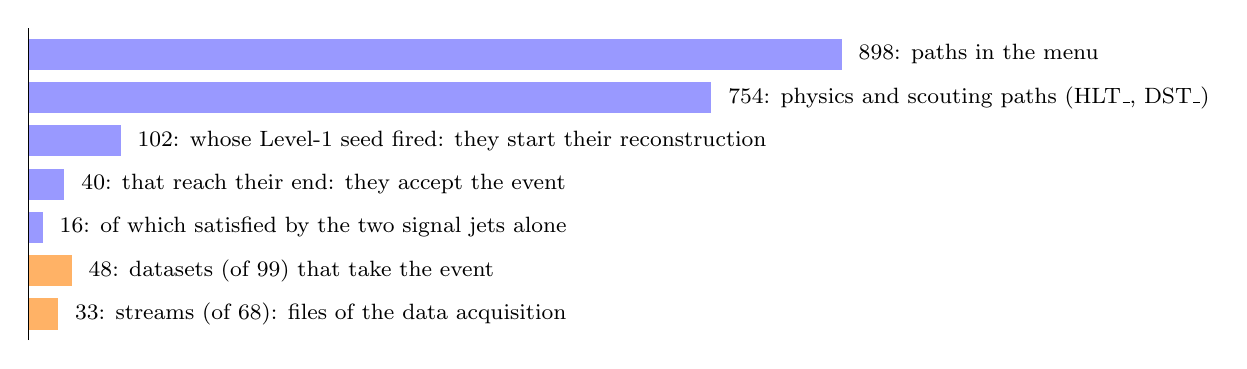
\begin{tikzpicture}[x=0.0115cm, y=0.55cm, font=\footnotesize]
\foreach \y/\v/\t in {6/898/{paths in the menu}, 5/754/{physics and scouting paths (\code{HLT\_}, \code{DST\_})},
  4/102/{whose Level-1 seed fired: they start their reconstruction}, 3/40/{that reach their end: they accept the event},
  2/16/{of which satisfied by the two signal jets alone}, 1/48/{datasets (of 99) that take the event},
  0/33/{streams (of 68): files of the data acquisition}}
{ \fill[\ifnum\y>1 blue!40\else orange!60\fi] (0,\y-0.36) rectangle (\v,\y+0.36);
  \node[anchor=west] at (\v+8,\y) {\v: \t}; }
\path (0,0) -- (940,0);
\draw (0,-0.6) -- (0,6.6);
\end{tikzpicture}
\caption{Step 5, the decision as a funnel (\code{ledger\_13\_HLT.txt}, section 5). The length of a bar is the number
of paths (blue) or of datasets and streams (orange).}
\label{fig:13_funnel}
\end{figure}

\textbf{The record of the decision.} What an analysis finds in the file about \code{HLT\_PFJet110}: its bit in
\code{TriggerResults}, and in \code{hltTriggerSummaryAOD} the objects of its three filters with \code{saveTags}, as
(\pt, $\eta$, $\phi$) (\path{hlt_13_HLT.log}, lines \code{filter:}):

\begin{lstlisting}[style=txt]
path: name=HLT_PFJet110_v13 accept=1 stage=accept seedFired=1 last=hltBoolEnd lastIndex=208 nModules=209
filter: label=hltL1sSingleJet90     type=HLTL1TSeed  n=2 | L1Jet(136.0,-3.74,1.00) L1Jet(108.5,-1.52,-1.98)
filter: label=hltSingleAK4CaloJet80 type=HLT1CaloJet n=2 | Jet(118.5,-3.72,0.96) Jet(93.3,-1.58,-2.08)
filter: label=hltSinglePFJet110     type=HLT1PFJet   n=1 | Jet(126.7,-3.77,0.96)
\end{lstlisting}

\noindent Each step of the path narrowed the list: two Level-1 jets, two calo jets, one PF jet. An analysis that uses
this trigger checks that its own jet is close to that last object, and measures the efficiency of the path with
events of a lower, prescaled path, \code{HLT\_PFJet80} for example, in which the jet above $110\GeV$ was not required.

\textbf{What else accepts it.} 40 of the 754 paths (table~\ref{tab:13_accepted}, figure~\ref{fig:13_funnel}). Sixteen are jet paths satisfied by
the two signal jets. Two need an object the hard collision did not make: \code{HLT\_Mu3\_PFJet40} finds the muon of
chapter~\ref{ch:12_L1T}, the kaon of a pileup collision that decayed in flight, now reconstructed by the HLT
(with $3.1\GeV$ by the muon chambers alone, \code{hltL2Muons}, then $3.0\GeV$ with the tracker,
\code{hltIterL3MuonCandidates}), and pairs it with the $b$ jet; \code{HLT\_CaloMET90\_NotCleaned} finds a missing
transverse energy of $138.5\GeV$ in the towers, where the neutrino carries $37.5\GeV$. Three paths ask only for their
Level-1 seed. Twelve select nothing at all: zero bias, random, ``physics'' (any event), calibration and monitoring
paths, which in data run prescaled or on special events. Seven are scouting paths (\code{DST\_}): they save not the
raw event but a compact list of HLT objects, at a high rate; four of them are seeded by the CICADA anomaly score of
chapter~\ref{ch:12_L1T}.

\begin{table}[!htb]
\centering\small
\caption{Step 5: the 40 \code{HLT\_} and \code{DST\_} paths that accept the event, by what satisfies them
(\code{ledger\_13\_HLT.txt}, section 5).}
\label{tab:13_accepted}
\begin{tabular}{@{}>{\raggedright\arraybackslash}p{4.1cm} c >{\raggedright\arraybackslash}p{9.6cm}@{}}
\toprule
satisfied by & paths & which \\
\midrule
the two signal jets & 16 & \code{HLT\_PFJet40}, \code{60}, \code{80}, \code{110}; \code{PFJetFwd40}, \code{60}, \code{80}; \code{AK8PFJet40}, \code{60}, \code{80}; \code{AK8PFJetFwd40}, \code{60}, \code{80}; \code{DiPFJetAve40}, \code{60}, \code{80} \\
a pileup object & 2 & \code{HLT\_Mu3\_PFJet40} (the muon of a pileup kaon), \code{HLT\_CaloMET90\_NotCleaned} ($138.5\GeV$) \\
the L1 seed alone & 3 & \code{HLT\_L1SingleMuCosmics}, \code{HLT\_L1ETMHadSeeds}, \code{HLT\_L1AlwaysTrue} \\
no object & 12 & \code{HLT\_ZeroBias} (and \code{\_Alignment}, \code{\_Beamspot}), \code{HLT\_Physics}, \code{HLT\_Random}, \code{HLT\_EphemeralPhysics}, \code{HLT\_EphemeralZeroBias}, \code{HLT\_EcalCalibration}, \code{HLT\_HcalCalibration}, \code{HLT\_HcalNZS}, \code{HLT\_HcalPhiSym}, \code{HLT\_PPSRandom} \\
scouting & 7 & \code{DST\_PFScouting\_CICADA*} (4), \code{DST\_PFScouting\_ZeroBias}, \code{DST\_ZeroBias}, \code{DST\_Physics} \\
\bottomrule
\end{tabular}
\end{table}

\textbf{Where the event goes.} 48 of the 99 datasets and 33 of the 68 streams accept it. For physics the ones that
matter are \code{JetMET0} and \code{JetMET1} (18 of their 150 paths fired; the two are copies that split the rate),
\code{Muon0} and \code{Muon1} (one path of 129, \code{HLT\_Mu3\_PFJet40}: the event would be in the muon dataset
because of a pileup kaon), \code{ZeroBias}, and the scouting dataset \code{ScoutingPFRun3}. The jet analysis this
book is heading to reads \code{JetMET}: the stream \code{PhysicsJetMET0}, the dataset \code{JetMET0}, the trigger bit
\code{HLT\_PFJet110\_v13} with the $\bar b$ jet as its object.

\FloatBarrier
\section{Ledger and display}

A checkpoint has a ledger in two parts. The first is what the HLT \emph{sees}, step by step
(table~\ref{tab:13_ledger}, top), with the two jets of the signal followed through every step
(figure~\ref{fig:13_twojets}); nothing of it is added to or removed from the recorded event, whose raw data are those
of step~1. The second is the decision (bottom).

\begin{table}[!htb]
\centering\small
\caption{The ledger of the High Level Trigger (\code{ledger\_13\_HLT.txt}). Top: what each step reconstructs.
Middle: the two jets of the signal. Bottom: the decision.}
\label{tab:13_ledger}
\begin{tabular}{@{}p{7.0cm} r >{\raggedright\arraybackslash}p{4.4cm}@{}}
\toprule
\multicolumn{3}{@{}l}{\emph{what the HLT sees}} \\
step 1: raw event (678 FEDs) & 1862 kB & strip tracker 54\,\% \\
step 1: Level-1 algorithms fired / jets unpacked & 63 / 9 & as in chapter~\ref{ch:12_L1T} \\
step 2: rec-hits, $\sum E_{\mathrm T}$ & 3198.9 GeV & 11\,193 rec-hits \\
step 2: towers, $\sum E_{\mathrm T}$ & 2842.9 GeV & 2051 towers; HF 1617.2 \\
step 2: $\rho$ (calorimeter) & 36.3 GeV & per unit area \\
step 2: calo jets above 30 GeV, raw / corrected & 23 / 2 & of 190 \\
step 3: pixel tracks / pixel vertices / kept & 2981 / 31 / 1 & 68 + 1 collisions \\
step 3: full tracks, $\sum\pt$ & 116, 179.5 GeV & of the signal vertex: 61, 121.8 \\
step 3: PF vertices & 1 & $7\um$ from the signal \\
step 4: PF candidates, $\sum\pt$ & 1366, 2655.8 GeV & HF: 783 \\
step 4: $\rho$ (particle flow) & 36.7 GeV & per unit area \\
step 4: PF jets above 30 GeV, raw / corrected & 13 / 2 & of 192 \\
\midrule
\multicolumn{3}{@{}l}{\emph{the two signal jets: $b$ ($\eta=-1.59$) and $\bar b$ ($\eta=-3.75$), \pt{} in GeV}} \\
generator jet (visible particles) & 117.8 (79.8) / 115.9 & chapter~\ref{ch:07_GenJet} \\
Level-1 jet & 108.5 / 136.0 & chapter~\ref{ch:12_L1T} \\
calo jet, raw $\rightarrow$ corrected & 70.9 $\rightarrow$ 93.3 / 163.5 $\rightarrow$ 118.5 & step 2 \\
tracks in the jet & 7, 50.1 / 0 & step 3 \\
PF jet, raw $\rightarrow$ corrected & 83.7 $\rightarrow$ 86.7 / 156.8 $\rightarrow$ 126.7 & step 4 \\
\midrule
\multicolumn{3}{@{}l}{\emph{decision}} \\
paths \code{HLT\_} and \code{DST\_} & 754 & \\
\quad stopped by the L1 seed / a prescale / a filter & 652 / 0 / 62 & \\
\quad accepting the event & 40 & 16 on the signal jets alone \\
\code{HLT\_PFJet110}, the path of the book & accepted & by 16.7 GeV, on the $\bar b$ jet \\
highest single-jet threshold passed & 110 & 140 failed by 13.3 GeV \\
datasets / streams & 48 / 33 & \code{JetMET0}, \code{PhysicsJetMET0} \\
\bottomrule
\end{tabular}
\end{table}

Read downwards, the ledger says what each step of the HLT is for. The calorimeters see $2843\GeV$ of towers; the
pileup subtraction leaves two jets, which are the signal. The tracker sees 2981 pixel tracks; the HLT builds its 116
full tracks around one collision, which is the signal. Particle flow brings the $b$ jet to $86.7\GeV$, near its visible energy, and
cannot help the $\bar b$ jet, which no tracker sees. The decision then turns on that jet: \code{HLT\_PFJet110} fires
because the HF jet is measured at $126.7\GeV$, 9\,\% above its true \pt. Of the 40 paths that accept the event, 16
are satisfied by the two signal jets alone, and the jet path of the book is one of them.

\paragraph{What the year changed.} With the 2024 settings (the first version of this chapter; the companion compares
the two step by step) the menu had to be cut to 861 paths, and 41 of 717 accepted the event. With 2025 the menu runs
whole and 40 of 754 accept: the VBF, multijet and electron paths do not even start, because their Level-1 seeds,
fired in 2024 by the ring-28 jets and a cluster of $8\GeV$, did not fire; one CICADA scouting path is lost with
\code{L1\_CICADA\_VTight}. The path of the book is untouched: the $\bar b$ jet moved from 125.9 to $126.7\GeV$ and
\code{HLT\_PFJet110} accepts by $16.7\GeV$ instead of $15.9\GeV$. Table~\ref{tab:13_years} puts the two side by side.

\begin{table}[!htb]
\centering\small
\caption{The same event through the HLT with the 2024 and the 2025 settings of the release (the 2024 numbers are
those of the first version of this chapter; companion, last section). Values in GeV unless stated.}
\label{tab:13_years}
\begin{tabular}{@{}l rr >{\raggedright\arraybackslash}p{5.6cm}@{}}
\toprule
 & 2024 & 2025 & why \\
\midrule
HLT menu, paths run & 861 & 898 & 2024: 37 removed, their seeds not in the Level-1 menu \\
Level-1 algorithms fired / L1 jets & 57 / 12 & 63 / 9 & no jet in tower ring 28 (chapter~\ref{ch:12_L1T}) \\
raw event, kB (ECAL) & 1929 (173) & 1862 (104) & ECAL barrel zero suppression (chapter~\ref{ch:11_DIGI}) \\
ECAL barrel rec-hits & 2039 & 956 & the same \\
towers, $\sum E_{\mathrm T}$ & 3085.5 & 2842.9 & the two ECAL changes of chapter~\ref{ch:11_DIGI} \\
$\rho$ calorimeter / particle flow & 40.0 / 36.4 & 36.3 / 36.7 & \\
calo jets $b$ / $\bar b$, corrected & 88.5 / 113.4 & 93.3 / 118.5 & \\
full tracks / pixel vertices & 115 / 27 & 116 / 31 & pixel digis and templates of 2025 \\
PF jets $b$ / $\bar b$, corrected & 80.3 / 125.9 & 86.7 / 126.7 & $b$: one track of $11\GeV$ more \\
paths started / accepted & 124 / 41 & 102 / 40 & VBF, multijet, electron seeds not fired \\
\code{HLT\_PFJet110}, margin & 15.9 & 16.7 & \\
datasets / streams & 47 / 32 & 48 / 33 & \\
\bottomrule
\end{tabular}
\end{table}

\begin{figure}[!htb]
\centering
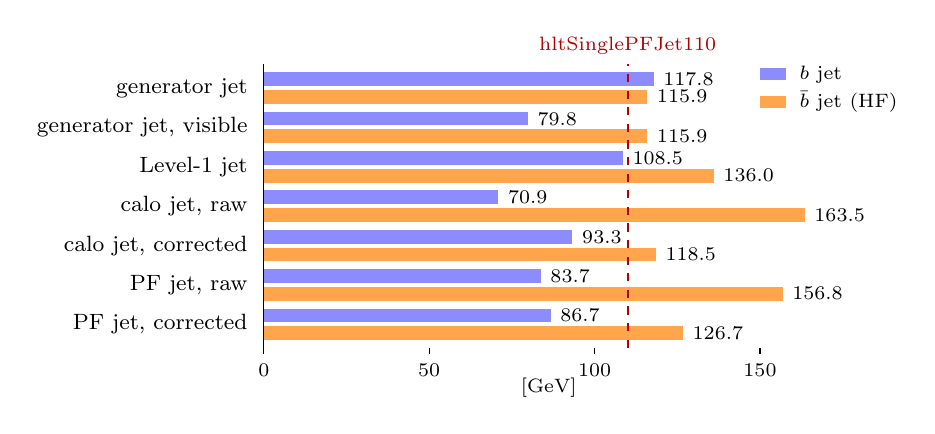
\begin{tikzpicture}[x=0.042cm, y=0.5cm, font=\footnotesize]
\foreach \y/\t/\b/\bb in {6/{generator jet}/117.8/115.9, 5/{generator jet, visible}/79.8/115.9, 4/{Level-1 jet}/108.5/136.0,
                          3/{calo jet, raw}/70.9/163.5, 2/{calo jet, corrected}/93.3/118.5, 1/{PF jet, raw}/83.7/156.8, 0/{PF jet, corrected}/86.7/126.7}
{ \node[anchor=east] at (-2,\y) {\t};
  \fill[blue!45] (0,\y+0.05) rectangle (\b,\y+0.4); \node[anchor=west, font=\scriptsize] at (\b,\y+0.22) {\b};
  \fill[orange!70] (0,\y-0.4) rectangle (\bb,\y-0.05); \node[anchor=west, font=\scriptsize] at (\bb,\y-0.22) {\bb}; }
\draw (0,-0.6) -- (0,6.6);
\draw[red!70!black, dashed, thick] (110,-0.6) -- (110,6.6) node[above, font=\scriptsize] {\code{hltSinglePFJet110}};
\foreach \x in {0,50,100,150} { \draw (\x,-0.6) -- (\x,-0.75) node[below, font=\scriptsize] {\x}; }
\node[font=\scriptsize] at (85,-1.6) {\pt{} [GeV]};
\fill[blue!45] (150,6.2) rectangle (158,6.5); \node[anchor=west, font=\scriptsize] at (159,6.35) {$b$ jet};
\fill[orange!70] (150,5.5) rectangle (158,5.8); \node[anchor=west, font=\scriptsize] at (159,5.65) {$\bar b$ jet (HF)};
\end{tikzpicture}
\caption{The two jets of the signal through the trigger (table~\ref{tab:13_ledger}, middle). The $b$ jet loses its
neutrino and never comes back above $110\GeV$; the $\bar b$ jet, in the HF, is measured above its true \pt{} at every
step and carries the decision.}
\label{fig:13_twojets}
\end{figure}

Figure~\ref{fig:13_objects} is the event as the HLT records it: the objects of the filters of the paths that
accepted it. Compare it with figure~\ref{fig:12_objects}, the 34 objects that the Level-1 trigger handed over, and
with figure~\ref{fig:11_mixed}, the $544\,407$ digis of the same event: what is left are the two jets the journey has
followed since chapter~\ref{ch:01_ME}.

\begin{figure}[!htb]
\centering
\includegraphics[width=0.93\textwidth]{13_HLT/out/hlt_13_HLT_seed_objects_run1_event1.png}
\caption{The event as the HLT records it (\code{hlt\_13\_HLT\_seed\_objects\_run1\_event1.png}): the objects of the last
filter of each accepted \code{HLT\_} path, from \code{hltTriggerSummaryAOD}. Red squares: AK4 PF jets ($126.7$ and
$86.7\GeV$); open orange squares: AK8 PF jets; the tick on the left edge: the direction of the calorimeter missing
transverse energy. Magenta circles: the two generator jets. The right panel lists the physics datasets.}
\label{fig:13_objects}
\end{figure}

\FloatBarrier
\section{Open problems for Phase-2}

The Phase-2 HLT will receive 750\,kHz from the Level-1 trigger instead of 100\,kHz, at a pileup of 140 to 200, with
a new tracker, the HGCAL in the endcaps and a timing layer (MTD). Its menu in the release is \code{75e33}
(\path{HLTrigger/Configuration/python/HLT_75e33_cff.py} and the directory \path{HLT_75e33/}; \code{HLT:@relvalRun4}
in \path{Configuration/HLT/python/autoHLT.py}). What follows compares it with the Run-3 menu of this chapter, step by
step; every statement is a line of the release or of the global tag of the Phase-2 workflows,
\code{150X\_mcRun4\_realistic\_v1} (\path{Configuration/AlCa/python/autoCond.py}, line 111).

\textbf{An event like ours has no Phase-2 path.} The schedule of \code{75e33} (line 353 of the \code{\_cff}) has 54
entries: 32 \code{HLT\_}, 16 \code{L1T\_} (Level-1 objects cut at offline-equivalent thresholds), 4 \code{MC\_}, the
final path and an endpath, against the 898 paths of the 2025 menu. Its jet and energy-sum paths are \code{HLT\_AK4PFPuppiJet520} (seed \code{pSinglePuppiJet230}),
\code{HLT\_PFPuppiHT1070}, \code{HLT\_PFPuppiMETTypeOne140\_PFPuppiMHT140}, two double-jet paths with two $b$ tags
(two jets above $128\GeV$ with $\abseta<2.4$ and $\Delta\eta<1.6$, \path{hltDoublePFPuppiJets128MaxEta2p4_cfi.py}) and
four four-jet paths with three $b$ tags. There is no ladder of prescaled single-jet paths like \code{HLT\_PFJet40}
\ldots{} \code{450}, no forward jet path, no dijet-average path and no HF calibration path like
\code{HLT\_DiPFJetAve100\_HFJEC}. The paths that the jet energy scale and the trigger efficiencies are measured with
in Run~3, the 16 that accepted our event among them, are not written yet; and a $b\bar b$ pair with a jet in the HF
fails even the $b$-tag paths, which require $\abseta<2.4$ for both jets.

\textbf{The pileup subtraction of the Phase-2 HLT jets is an identity.} The jets of the Phase-2 HLT are PUPPI jets,
corrected in three levels with the payload \code{AK4PFPuppiHLT} (\path{HLT_75e33/modules/hltAK4PFPuppiJetCorrectorL1_cfi.py}:
\code{L1FastjetCorrectorProducer}, $\rho$ from \code{hltFixedGridRhoFastjetAll}, made of all PF candidates). In the
global tag that payload is \code{JetCorrectorParametersCollection\_Phase2Spring23ticlv4\_MC\_AK4PFPuppiHLT\_v1}, one
interval of validity written on 21 September 2023, and in it the L1FastJet level and the L3Absolute level both have
the formula ``1'' (\code{conddb dump} of the payload): the menu computes $\rho$ and runs a corrector that multiplies by
one. PUPPI removes the pileup particle by particle, so no offset may be the intention, but then a jet's response
rests on L2Relative alone, which has 19 bins of $\eta$ from $-5.2$ to $5.2$ (the Run-3 payload of this chapter has
82 bins of $\eta$, and 118 cells of $\eta\times\phi$). The name says ``ticlv4''; the menu already carries the
\code{ticl\_v5} alternative of the HGCAL reconstruction (\path{HLT_75e33/sequences/HLTIterTICLSequence_cfi.py}). The
same global tag gives the Run-3 HLT labels \code{AK4PFHLT} and \code{AK4CaloHLT} as \code{Run3Summer21} payloads.

\textbf{The pileup estimate of PUPPI is a count of pixel clusters, and in the HF it has no tracks.}
\path{HLT_75e33/modules/hltPFPuppi_cfi.py} has three regions: $\abseta<2.5$, $2.5<\abseta<3.5$ and
$3.5<\abseta<10$. In the first two the neutral threshold grows with the pileup (\code{MinNeutralPt} 0.5105 and
$0.821\GeV$ plus a slope of $9.51\times10^{-6}$ and $1.902\times10^{-5}$), and the pileup is measured by the number of
pixel clusters (\code{PUProxyValue = hltPixelClustersMultiplicity}), not by vertices. In the last region,
\code{useCharged = False} and a neutral particle needs $3.656\GeV$. Our $\bar b$ jet is in that region: 17 HF
particles of which, at PU 200, PUPPI can only cut the soft ones. The file has no comment, no date and no reference to
the sample its numbers were fitted on. The HF calibration of particle flow is off in both menus
(\code{calibHF\_use = False}, \path{HLT_75e33/modules/hltParticleFlowTmpBarrel_cfi.py}, line 121, as in
\code{hltParticleFlow} of the 2025 menu), and the Phase-2 particle flow reads the hadron calibration with the empty label
(line 122), which in the Phase-2 global tag is \code{PFCalibration\_Run3\_mc\_offline}: an offline Run-3 calibration,
where the Run-3 HLT reads its own (\code{calibrationsLabel = "HLT"}, \code{PFCalibration\_Run3\_2024\_online\_v1} in our
global tag).

\textbf{The tracking reconstructs every collision, without the timing layer.} Step~3 showed that the Run-3 HLT keeps
one pixel vertex of 31 (\code{hltTrimmedPixelVertices}, \code{fractionSumPt2 = 0.3}) and builds full tracks only
around it. In Phase-2 the seeds of the first iteration are all the pixel tracks, with no vertex
(\path{HLT_75e33/modules/hltInitialStepSeeds_cfi.py}: \code{InputVertexCollection = ""}, \code{usePV = False}); the only
vertex trimmer of the menu is in a muon path. At PU 200 the full tracking of every collision is the price of not
choosing the hard one too early. The primary vertices are found in $z$ only: \code{DA\_vect}, \code{useTiming =
False} (\path{hltOfflinePrimaryVertices_cfi.py}, line 22), no track times, although the era includes the timing layer
(\code{phase2\_timing}, \code{phase2\_timing\_layer}). The timing was the argument for the MTD at 200 collisions per
crossing.

\textbf{No cheap cut before the expensive steps.} A Run-3 jet path cuts on calo jets (step~2) before it pays for the
tracking. The Phase-2 jet paths go from the Level-1 seed (\code{PathStatusFilter} on a Phase-2 global-trigger
algorithm) to the full reconstruction and cut only on the PUPPI jets
(\path{HLT_75e33/paths/HLT_AK4PFPuppiJet520_cfi.py}); the calo jets of the menu serve only the vertex sorting. With
750\,kHz of input, every seeded event pays for tracking, HGCAL clustering and PUPPI.

\textbf{What the menu itself says.} The comments of \code{75e33} are few, and they are about unfinished business:
``Removed temporarily until final decision on L1T tau Phase-2'' (line 411, the two tau paths),
``Run3 thresholds. Will be overwritten with valid aging customisation'' (the HCAL thresholds of the e/$\gamma$
$H/E$, \path{hltEgammaHoverEL1Seeded_cfi.py}), ``Probably need to move elsewhere in the final setup''
(\path{HLTInitialStepSequence_cfi.py}). And the Run-3 lesson of this chapter applies to Phase-2 as well: a menu works
only with the Level-1 menu it was written for. The 2024 version of this chapter ran the 2025 HLT menu on the 2024
Level-1 decision, and could do so only after 30 of its seed algorithms were removed; the release simulates 2024 with a
fake HLT menu (\code{relval2024 : Fake2}). A Phase-2 study needs the Phase-2 HLT menu and the Phase-2 Level-1 menu of the same
date; the release has one of each, \code{75e33} and \code{step1\_2024}, the ``first prototype menu'' of
chapter~\ref{ch:12_L1T}.
